\documentclass[12pt, oneside]{article}   	% use "amsart" instead of "article" for AMSLaTeX format

%%%%%%%%%%%%%%%%%%%%%%%%%%%%%%%%%%%%%%%%%%%%%%%%%%%%
% set up packages, geometry
%%%%%%%%%%%%%%%%%%%%%%%%%%%%%%%%%%%%%%%%%%%%%%%%%%%%
\usepackage{geometry, textcomp, amsmath, graphicx, amssymb,fancyhdr,subcaption,bm}                
	
\geometry{letterpaper, marginparwidth=60pt}                   		
\usepackage[superscript,noadjust]{cite} % puts dash in citations to abbreviate
%\usepackage [autostyle, english = american]{csquotes} % sets US-style quotes
%\MakeOuterQuote{"} % sets quote style

\usepackage{hyperref}
\hypersetup{
    colorlinks=true,
    linkcolor=blue,
    filecolor=magenta,      
    urlcolor=cyan,
}

\usepackage{etoolbox}
\AtBeginEnvironment{quote}{\small}

\usepackage{float,color}

\usepackage{pgf, tikz, eqnarray}
\usetikzlibrary{arrows, automata}
%%%%%%%%%%%%%%%%%%%%%%%%%%%%%%%%%%%%%%%%%%%%%%%%%%%%

%%%%%%%%%%%%%%%%%%%%%%%%%%%%%%%%%%%%%%%%%%%%%%%%%%%%
\pagestyle{plain}                                                      %%
%%%%%%%%%% EXAFT 1in MARGINS %%%%%%%                                   %%
\setlength{\textwidth}{6.5in}     %%                                   %%
\setlength{\oddsidemargin}{0in}   %% (It is recommended that you       %%
\setlength{\evensidemargin}{0in}  %%  not change these parameters,     %%
\setlength{\textheight}{8.5in}    %%  at the risk of having your       %%
\setlength{\topmargin}{0in}       %%  proposal dismissed on the basis  %%
\setlength{\headheight}{0in}      %%  of incorrect formatting!!!)      %%
\setlength{\headsep}{0in}         %%                                   %%
\setlength{\footskip}{.5in}       %%                                   %%
%%%%%%%%%%%%%%%%%%%%%%%%%%%%%%%%%%%%                                   %%		

%%%%%%%%%%%%%
% DEFINE CODE BLOCK
%%%%%%%%%%%%%
\usepackage{listings}

\definecolor{dkgreen}{rgb}{0,0.6,0}
\definecolor{gray}{rgb}{0.5,0.5,0.5}
\definecolor{mauve}{rgb}{0.58,0,0.82}

\lstset{frame=tb,
  language=R,
  aboveskip=3mm,
  belowskip=3mm,
  showstringspaces=false,
  columns=flexible,
  basicstyle={\small\ttfamily},
  numbers=none,
  numberstyle=\tiny\color{gray},
 % keywordstyle=\color{blue},
  commentstyle=\color{dkgreen},
  stringstyle=\color{mauve},
  breaklines=true,
  breakatwhitespace=true,
  tabsize=3,
  otherkeywords={0,1,2,3,4,5,6,7,8,9},
  deletekeywords={data,frame,length,as,character,dunif,ps},
}

\begin{document} 

\section*{Control Problems} \label{mathrefs}

\noindent We can formulate our control problem generally as the following system of differential equations. We can express the state variables that compose $\bm{x}(t)$ in compact form that expresses the state vectors as functions of the current state, time, and the control:

$$ \bm{x} = f(\bm{x}(t),\bm{u}(t)) $$ \noindent or $$ \frac{d\bm{x}(t)}{dt} = f(\bm{x},t,\bm{u}(t)). $$ 

\noindent where the function(s) $f(\bm{x},t,{u})$ are continuous, differentiable functions of vectors $\bm{x}$ and $\bm{u}$ and variable $t$. The state variables $\bm{x}=\bm{x}(t)$ describe the state of the system as a function of time $t$. The system of state equations describes how the system changes from its initial states $bm{x}(0)$ under the controls $\bm{u}=\bm{u}(x)$. The final time $T$ is called the time horizon. \\

\noindent For a given control $\bm{u}(t)$, $0\leq t \leq T$, the solution $\bm{x}(t)$ is the response. We may want to consider the functions $\bm{u}(t)$ that are admissible controls. This class of functions $U$ is defined to be the class of all piecewise-continuous real functions $u(t)$ defined for $0\leq t \leq T$ and satisfying $u(t) \in U_t$ where $U_t$ is a given interval called the control set. \\

\noindent Many problems may also involve a terminal condition

$$ x(T) = x_T $$ 

\noindent A feasible control is then any admissible control such that the response satisfies this terminal condition as well as the initial conditions. \\

\noindent The basic issue in our optimal control problem is to find a feasible control $\bm{u}(t)$ that maximizes $J[\bm{u}]$. This would be the optimal control. 

$$ J[u] = \int_{t_0}^{t_f} g[\bm{x}(t), t, \bm{u}(t)] dt $$

\noindent where $g[\bm{x}(t), t, \bm{u}(t)]$ is a given, continuously differentiable function that represents the response to $u(t)$. The \textit{maximum principle} gives necessary conditions that must be met by an optimal control. \\

\noindent The maximum principle can be expressed in terms of the Hamiltonian:

\begin{align}
H[\bm{x}(t), t, \bm{u}(t); \bm{\lambda}(t)] & = g[\bm{x}(t), t, \bm{u}(t)] + \bm{\lambda}(t) f[\bm{x}(t), t, \bm{u}(t)] \label{eq:1}  \\
H & = g + \lambda^T f \label{eq:1}  
\end{align}

\noindent [Q: is the $t$ in the f(...) a derivative?; p. 91 of Clark]

\noindent where $\bm{\lambda}(t)$ are unknown functions called adjoint variables. For a system where $\bm{u}(t)$ is the optimal control and $\bm{x}(t)$ is the associated response, the maximum principle asserts existence of $\bm{\lambda}(t)$ such that these equations are satisfied for all t, $0\leq t \leq T$: [not sure if these are vectors or not?]

\begin{align}
\frac{d\bm{\lambda}}{dt} & = - \frac{ \partial H}{\partial \bm{x}} = - \frac{ \partial g}{\partial \bm{x}} - \bm{\lambda}(t) \frac{ \partial f}{\partial \bm{x}} \label{eq:1}, \\
H[\bm{x}(t), t, \bm{u}(t); \bm{\lambda}(t)] & = \max_{\{u \in U_t\}} H[\bm{x}(t), t, \bm{u}(t); \bm{\lambda}(t)] \label{eq:1},
\end{align}

\noindent The first of these requirements are the adjoint equations. These are equivalent to equation (6) in King and Roughgarden (1982), $\dot{\bm{\lambda}}^T =  - \frac{ \partial H}{\partial \bm{x}} $. King and Roughgarden take $\bm{\lambda}(t_f)=0$ as an additional point to define the adjoint variables when there are no final values for the state variables. This is a key assumption that states the marginal fitness benefit of investing in growth or reproduction at the time horizon $t_f$ is zero. \\

\noindent The expression for $J[\bm{u}(t)]$ is maximized by the $ \bm{u}(t) $ that maximize H at every point in time, as is stated in the second of the requirements above. \\

\noindent In one dimension, the optimal control problem has three unknown functions $x(t)$, $u(t)$, and $\lambda(t)$. For these three functions, there are three equations: a state equation, an adjoint equation, and the maximum principle. The state and adjoint equations are first-order, differential equations. Solutions to these equations require initial or terminal conditions. [these are thus key; in Clark p. 92 they are the initial value $x(0)$ and terminal value $x(T)$] \\

\noindent In our version of the problem, each unknown function is a vector of length four. This means that the optimal control problem now has 12 unknown functions.

\section*{Meristem and biomass allocation: explanation} \label{mathrefs}

\noindent In our model, we partition photosynthate among four pools. These pools are meristems committed to vegetative growth ($G$), vegetative biomass ($V$), meristems committed to reproduction ($F$), and reproductive biomass ($R$). \\

\noindent Growth in a season ($0<t<T$) is represented by the following system of differential equations:

\begin{align}
\frac{dG}{dt} & = u_1(t) p(t) \label{eq:1}  \\
\frac{dV}{dt} & = u_2(t) p(t) \label{eq:2}   \\
\frac{dF}{dt} & = u_3(t) p(t) \label{eq:3}  \\
\frac{dR}{dt} & = u_4(t) p(t) \label{eq:4}  \end{align}

\noindent where the $u_i$s represent rates and $P(t)$ is the production function. We assume that all energy produced by photosynthesis is allocated to vegetative meristems, to vegetative growth, to reproductive meristems, or to reproduction. Meristems are allocated to either growth or flowering; no meristems remain undifferentiated. Initial reproductive biomass is zero. We represent this with the following diagram: \newline

 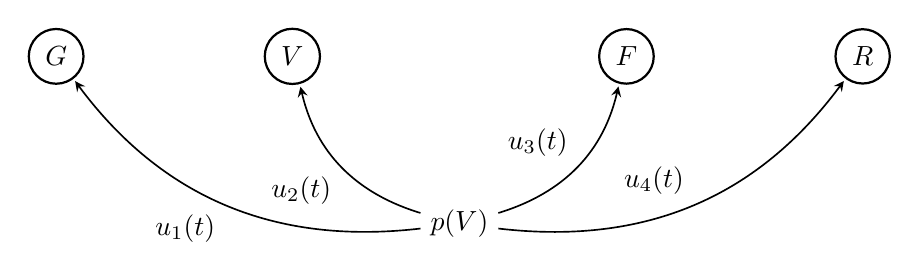
\begin{tikzpicture}[
            > = stealth, % arrow head style
            shorten > = 1pt, % don't touch arrow head to node
            auto,
            node distance = 3cm, % distance between nodes
            semithick % line style
        ]

        \tikzstyle{every state}=[
            draw = black,
            thick,
            fill = white,
            minimum size = 4mm
        ]F

        \node[] (P) {$p(V)$};
        
        \node[state] (V) [above left of=P] {$V$};
        \node[state] (G) [left of=V] {$G$};

        \node[state] (F) [above right of=P] {$F$};
        \node[state] (R) [right of=F] {$R$};        
      
        \path[->] (P) edge[bend left] node {$u_2(t)$} (V);
        \path[->] (P) edge[bend left] node {$u_1(t)$} (G);
        \draw[->] (P) edge[bend right,] node {$u_3(t)$} (F);
        \path[->] (P) edge[bend right] node {$u_4(t)$} (R);        
    \end{tikzpicture} \newline

\noindent Daily photosynthesis ($p(V)$) is a function of vegetative biomass. The plant starts from initial size $p(V(0))$ set by seed resources. Following Iwasa (200), we assume that daily biomass production (photosynthesis production, respiration cost) daily net production, is an increasing, saturating function of the vegetative biomass written as

\begin{equation} p(V) = \frac{aV}{1 + hV}. \label{eq:5}  \end{equation}

\noindent Photosynthate is allocated between vegetative meristem differentiation ($u_1(t)$), vegetative biomass ($u_2(t)$), reproductive meristem differentiation ($u_3(t)$) and reproductive biomass ($u_5(t)$). The model jump starts photosynthesis by setting an initial seed size but constraints on $u_2$ and $u_4$ (see below) limit production of vegetative biomass unless there is also allocation to meristems for growth and reproduction. Plants are modular and meristem differentiation and subsequent determination are necessary to add vegetative modules (phytomers: internode+node with leaf+axillary meristem bud). The arrow from meristem state (M) to meristems for growth (G) corresponds to determination and growth of vegetative organs (e.g. leaf expansion) and requires energy that limits accumulation in V. For example, a low rate of allocation to meristems for growth (low $u_1$) limits the allocation of photosynthate to V. \\

\noindent We impose the following constraints
\begin{align}
 u_1 + u_2 + u_3 + u_4 & = 1 \label{eq:6} \\ 
 u_i & \geq 0 \label{eq:7}  \\
 u_2 & \leq c u_1 \label{eq:8}  \\
 u_4 & \leq c u_3 \label{eq:9}  
\end{align} 

\noindent which can be interpreted as follows. All energy that gets produced is allocated to one of the four pools \textemdash the $u_i$s sum to one (Equation \ref{eq:6}). Energy flows in a one direction, and either energy is flowing in one of the paths or is not \textemdash allocation rates ($u_i$s) are zero or positive (Equation \ref{eq:7}). The rate of energy allocation to vegetative meristems constrains the rate of energy allocation to vegetative biomass \textemdash $u_2$ is less than or equal to $u_1$ multiplied by a constant $c$ that acts as a constraint (Equation \ref{eq:8}). Similarly, the rate of energy allocation to vegetative meristems constrains the rate of energy allocation to vegetative biomass \textemdash $u_4$ is less than or equal to $u_3$ multiplied by a constant $d$ that acts as a constraint (Equation \ref{eq:9}). These condition says that to allocate energy to biomass the plant must concurrently allocate energy to meristems. \\
    
\section*{Meristem and biomass allocation: control problem}

\noindent We can formulate our control problem as the following system of differential equations. Growth in a season ($0<t<T$) is represented by the following system of differential equations:
\begin{align}
\frac{dx_1}{dt} & = \frac{a x_2}{1 + h x_2} \times u_1(t) \label{eq:1}  \\
\frac{dx_2}{dt} & = \frac{a x_2}{1 + h x_2} \times u_2(t) \label{eq:2}   \\
\frac{dx_3}{dt} & = \frac{a x_2}{1 + h x_2} \times u_3(t) \label{eq:3}  \\
\frac{dx_4}{dt} & = \frac{a x_2}{1 + h x_2} \times u_4(t) \label{eq:4},
\end{align}

\noindent and 
\begin{align}
0 \leq t \leq T
\end{align}

\noindent with the following initial conditions
\begin{align}
x_1(0) & = x_0 \label{eq:1}  \\
x_2(0) & = x_0 \label{eq:1}  \\
x_3(0) & = x_0 \label{eq:1}  \\
x_4(0) & = x_0 \label{eq:1}.  
\end{align}

\noindent We impose the following constraints to define the class $U$ of admissible controls
\begin{align}
 u_1 + u_2 + u_3 + u_4 & = 1 \label{eq:6} \\ 
 u_i & \geq 0 \label{eq:7}  \\
 u_2 & \leq c u_1 \label{eq:8}  \\
 u_4 & \leq c u_3 \label{eq:9}  
\end{align}     

\section*{Optimization: implementation} \label{mathrefs}
\subsection*{Optimal control}

\noindent The state variables in the ODE are $G$, $V$, $F$, and $R$. The constants $a$ and $h$ are the parameters in the ODE. The values $c$ and $d$ are the constraints in the ODE. \\

\noindent We rewrite these as 

\begin{align}
 u_1 & = f_1(t) \label{eq:10} \\
 u_2 & = f_2(t) \label{eq:11} \\
 u_3 & = f_3(t) \label{eq:12} \\
 u_4 & = 1-(u_1+u_2+u_3) \label{eq:13} 
\end{align}

\noindent and build the constraints into the differential equations as 

\begin{align} 
u_2 & = \min(u_2, c*u_1) \label{eq:14}  \\
u_4 & = \min(u_1, d*u_3) \label{eq:15} 
 \end{align}

\subsection*{Constraint matrix}

\noindent See \url{https://cran.r-project.org/web/views/Optimization.html} for various R packages associated with optimization. \\ 

\noindent We are using linear programming to deal with our problem [this comes from notes to Lecture 1, Math 407, Jim Burke, UW]. Linear programming takes an optimization problem over $\mathbb{R}^n$ where the objective function is a linear function of the form 

\begin{align}
c_1 x_1 + c_2 x_2 + \dots + c_n x+n 
\end{align}

\noindent for some $c_i \in \mathbb{R}^n; i = 1,\dots,n $ and the region is a set of solutions subject to linear inequality and equality constraints

\begin{align}
a_{i1} x_i + a_{i2} x_2 + \dots + a_{in} x+n \leq \alpha_i ;  i = 1,\dots,s \\
\end{align}

\noindent and

\begin{align}
b_{i1} x_i + b_{i2} x_2 + \dots + b_{in} x+n = \beta_i ;  i = 1,\dots,r
\end{align}

\noindent These can be rewritten in compact form as

\begin{align}
 \mathrm{maximize} & \  c^Tx \\
 \mathrm{subject \ to} & \  Ax \leq \alpha \ \mathrm{and} \ Bx = \beta 
\end{align}

\noindent We can reformulate the optimization problem as follows. We are implementing a constrained optimization problem, as we have inequality constraints.  The constraint matrix comes from linear programming and defines the equations and inequalities that define the set of solutions. For optimization, we then constructed a constraint matrix with four blocks. We split the season $ \left[ 0,T \right] $ into $t$ time steps. \\

\noindent We implemented the constraints $ u_1+u_2+u_3 - 1 \leq 0 $ and that $u_4$ is positive as:

\[ A_{11}=
  \begin{bmatrix}
    -1		& 0 	 	& \ldots 	& 0  	 \\
    0 	 	& -1  	& \ddots 	& \vdots  \\
    \vdots   & \ddots 	& -1		& 0  \\
    0 		& \ldots 	& 0 		& -1  
  \end{bmatrix}_{ t \times t}
 \]
 
\[
A_{12}=
  \begin{bmatrix}
    -1		& 0 	 	& \ldots 	& 0  	 \\
    0 	 	& -1  	& \ddots 	& \vdots  \\
    \vdots   & \ddots 	& -1		& 0  \\
    0 		& \ldots 	& 0 		& -1  
  \end{bmatrix}_{ t \times t}
\]

\[
A_{13}=
  \begin{bmatrix}
    -1		& 0 	 	& \ldots 	& 0  	 \\
    0 	 	& -1  	& \ddots 	& \vdots  \\
    \vdots   & \ddots 	& -1		& 0  \\
    0 		& \ldots 	& 0 		& -1  
  \end{bmatrix}_{ t \times t}
\]

\[
A_1=
  \begin{bmatrix}
   A_{11} & A_{12} & A_{13}
   \end{bmatrix}_{t \times 3t}
\]

\[
b_1=
  \begin{bmatrix}
    -1 & -1 & \dots & -1
  \end{bmatrix}_{ 1 \times t }
\]

\noindent We implemented the constraint that $u_i $ be positive (??) as:

\[
A_2=
  \begin{bmatrix}
    1		& 0 	 	& \ldots 	& 0  	 \\
    0 	 	& 1  		& \ddots 	& \vdots  \\
    \vdots   & \ddots 	& 1		& 0  \\
    0 		& \ldots 	& 0 		& 1  
  \end{bmatrix}_{ 3t \times 3t}
\]

\[
b_2=
  \begin{bmatrix}
    0 & 0 & \dots & 0
  \end{bmatrix}_{ 1 \times 3t }
\]

\noindent Together 

\[
\bm{A} = \begin{bmatrix}
    A_1 & A_2 
\end{bmatrix}_{ 4t \times 3t }
\] 

\noindent and

\[
\bm{b} = \begin{bmatrix}
    b_1 & b_2 
\end{bmatrix}_{ 1 \times 4t }
\] 

\noindent These matrices define the following 

\begin{align}
A \bm{\theta} - \bm{b} \geq 0 
\end{align}

\noindent Our approach included only inequality constraints given by A and b. (meq=0 in the constrOptim function). We define our constraint as Ax greater than or equal to b, we don't have a second constraint for equality. Our objective function gives the output that we want to maximize/minimize. The variables are the inputs we control (?). The constraints are equations that limit the variables. The variables influence the objective function, and the constraints place limits on the domain of variables. In our case, the constraints limit the $u$ functions which are the variables that go into the objective function where the objective function integrates the system of DE over time.  \\

\iffalse
\noindent I've seen recommendations online that recommend augmented Lagrangian approach (alabama) rather than constrOptim. 

\subsection*{Optimization}

\begin{itemize}
\item initial conditions

\item Penalized optimization: use optim with a custom written penalizedfun and method=BFGS for initial guess

\item Check thetas from the fit and break if ??

\item Take initial guess and use constrained optimization to move the needle further. Uses optimfun, optimgrad (gradient function) and applies these to the ui and cis that are given as a matrix.

\item optimfun (in simple-optimalfuns)

\item Use some stop criteria to pick the stopping piont (combines Nelder Mead and BFGS)
\end{itemize}

\subsection*{Plotting}
take matrix of uis to calculate u4, plot uis and allocation
\fi


\end{document}